\RequirePackage{fix-cm}
\documentclass{article}
\usepackage[paperwidth=841mm,paperheight=1189mm,margin=18mm]{geometry}
\usepackage[utf8]{inputenc}
\pdfmapfile{+cm.map}
\pdfmapfile{+cmextra.map}
% Embed the metrically compatible Nimbus Sans faces for Helvetica text.
\pdfmapfile{+poster_helvetica.map}
\usepackage[scaled=0.92]{helvet}
\renewcommand{\familydefault}{\sfdefault}
\usepackage{amsmath,amssymb,graphicx,booktabs,xcolor,hyperref}
\pagestyle{empty}
\setlength{\parindent}{0pt}
\setlength{\parskip}{4mm}
\setlength{\fboxsep}{0pt}
\graphicspath{{figures/}}

% SFB 1294 poster template: up-blue, mathnat-blue, and up-grey.
\definecolor{upblue}{RGB}{0,48,94}
\definecolor{mathnatblue}{RGB}{0,128,181}
\definecolor{upgrey}{RGB}{193,211,224}
\definecolor{bodyink}{RGB}{17,43,62}
\pagecolor{upgrey}
\hypersetup{colorlinks=true,urlcolor=mathnatblue}

\newcommand{\card}[2]{%
  \par\noindent\colorbox{white}{%
    \parbox{\linewidth}{%
      \colorbox{mathnatblue}{%
        \parbox[c][19mm][c]{\linewidth}{%
          \hspace*{9mm}{\color{white}\bfseries\fontsize{37}{43}\selectfont #1}%
        }%
      }\par
      \vspace{7mm}
      \hspace*{9mm}\begin{minipage}{\dimexpr\linewidth-18mm\relax}
        \color{bodyink}\fontsize{27}{36}\selectfont
        #2
      \end{minipage}\par
      \vspace{8mm}
    }%
  }\par\vspace{11mm}%
}
\newcommand{\captiontext}[1]{{\fontsize{22}{28}\selectfont #1\par}}
\newcommand{\posterformula}{\fontsize{29}{37}\selectfont}

\begin{document}
\fontsize{27}{36}\selectfont

% Header follows the supplied SFB template: dark-blue logo panels and
% a cyan title panel. The two logos are vector conversions of supplied EPS.
\noindent\colorbox{upblue}{%
  \parbox[c][154mm][c]{0.20\textwidth}{%
    \centering\includegraphics[width=0.90\linewidth]{sfb_logo_negative.pdf}\par
    \vspace{7mm}{\color{white}\fontsize{24}{29}\selectfont
      SFB 1294\\Data Assimilation\par}%
  }%
}%
\colorbox{mathnatblue}{%
  \parbox[c][154mm][c]{0.60\textwidth}{%
    \hspace*{17mm}\begin{minipage}{\dimexpr\linewidth-34mm\relax}
      {\color{white}\bfseries\fontsize{68}{77}\selectfont
       Soft-ramp links for binned Poisson\\intensity inference\par}
      \vspace{6mm}
      {\color{white}\fontsize{30}{38}\selectfont
       Gaussian-mixture augmentation for a spatial latent field\par}
      \vspace{6mm}
      {\color{white}\fontsize{28}{36}\selectfont
       Cristina O. Ch\'avez Chong\quad Toni Ludo\quad Matthias Holschneider\par}
    \end{minipage}%
  }%
}%
\colorbox{upblue}{%
  \parbox[c][154mm][c]{0.20\textwidth}{%
    \centering\includegraphics[width=0.62\linewidth]{up_logo_white.pdf}\par
    \vspace{2mm}{\color{white}\fontsize{23}{29}\selectfont
      University of Potsdam\par}%
  }%
}

\vspace{12mm}
\noindent
\begin{minipage}[t]{0.483\textwidth}
\vspace{0pt}
\card{Problem: a spatial background rate}{%
In ETAS, the conditional event rate separates into a spatial background
component and triggering from previous earthquakes:
{\posterformula
\[
\lambda_{\rm ETAS}(t,x\mid\mathcal H_t)
=\mu(x)+\sum_{t_j<t}\varphi_j(t,x).
\]
}
We focus on $\mu(x)$. Given background labels or a declustered catalogue,
cell $C_i$ contains $n_i^{\rm bg}$ background events, with
{\posterformula
\[
\Lambda_i=\int_0^T\!\int_{C_i}\mu(x)\,dx\,dt,
\qquad n_i^{\rm bg}\mid f_i\sim\operatorname{Poisson}(\Lambda_i).
\]
}%
}

\card{Model: an unbounded soft-ramp link}{%
We use $\Lambda_i=L_\kappa(f_i)$ on a regular grid, with time and cell
area absorbed into the expected-count parameterization:
{\posterformula
\[
f\sim\mathcal N(m,Q^{-1}),\qquad
L_\kappa(f)=\kappa^{-1}\log(1+e^{\kappa f}),\quad\kappa>0.
\]
}
The sigmoid model $\lambda_0\sigma(f)$ has a fixed upper rate;
$L_\kappa$ remains positive and unbounded.
\begin{center}
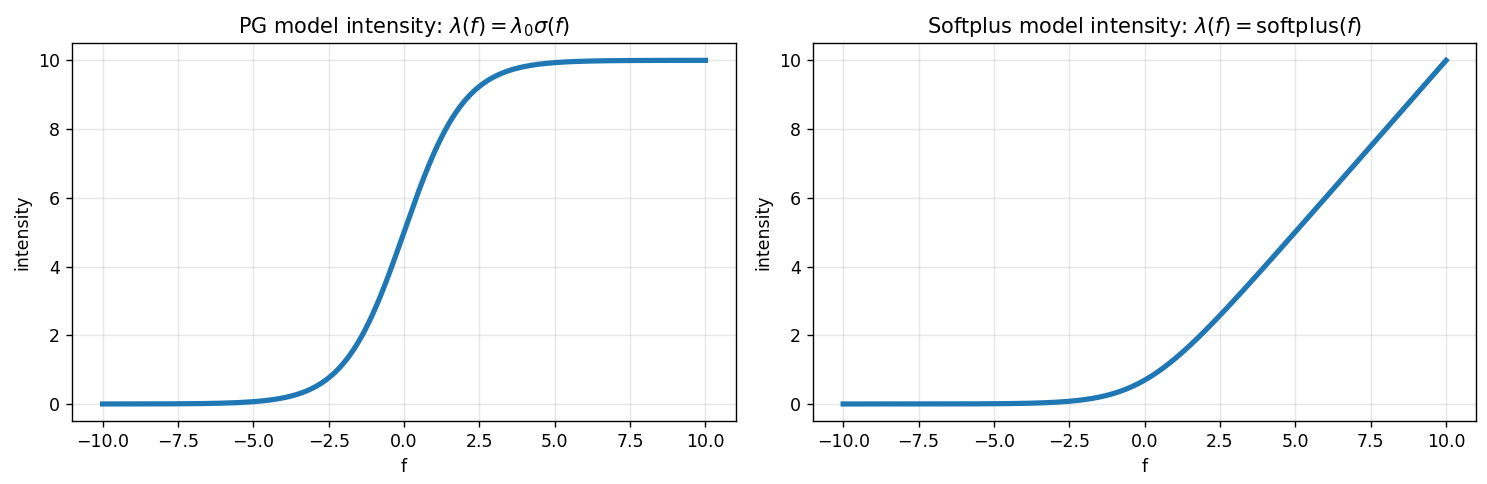
\includegraphics[width=0.99\linewidth]{link_functions.png}
\end{center}
\vspace{-3mm}
\captiontext{The link-function comparison from the supplied presentation.}
}

\card{Effect of the sharpness parameter}{%
The parameter $\kappa$ changes the transition around $f=0$.
For large $\kappa$, the soft-ramp approaches $\max(0,f)$:
\begin{center}
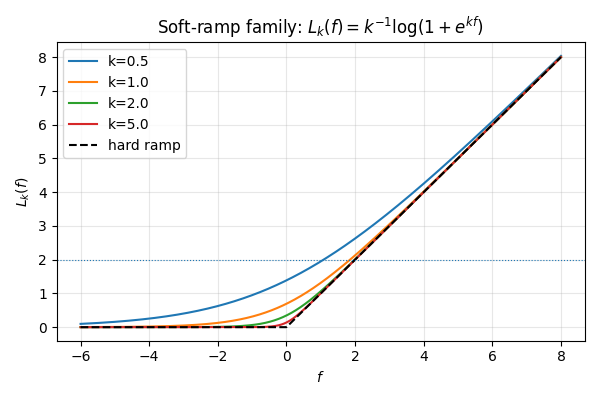
\includegraphics[width=0.63\linewidth]{soft_ramp_family.png}
\end{center}
\vspace{-3mm}
\captiontext{A smaller $\kappa$ gives a smoother transition.}
}

\card{Likelihood approximation}{%
For a count $n$, approximate the non-Gaussian likelihood in the latent
variable $f$ by a finite positive Gaussian mixture:
{\posterformula
\[
\ell_n(f)\propto L_\kappa(f)^n e^{-L_\kappa(f)}
\ \approx\ \sum_{r=1}^{R_n}w_{nr}\,
\mathcal N(f;m_{nr},s_n^2),\qquad w_{nr}\geq0.
\]
}
Components for the same count share a width $s_n$.
\begin{center}
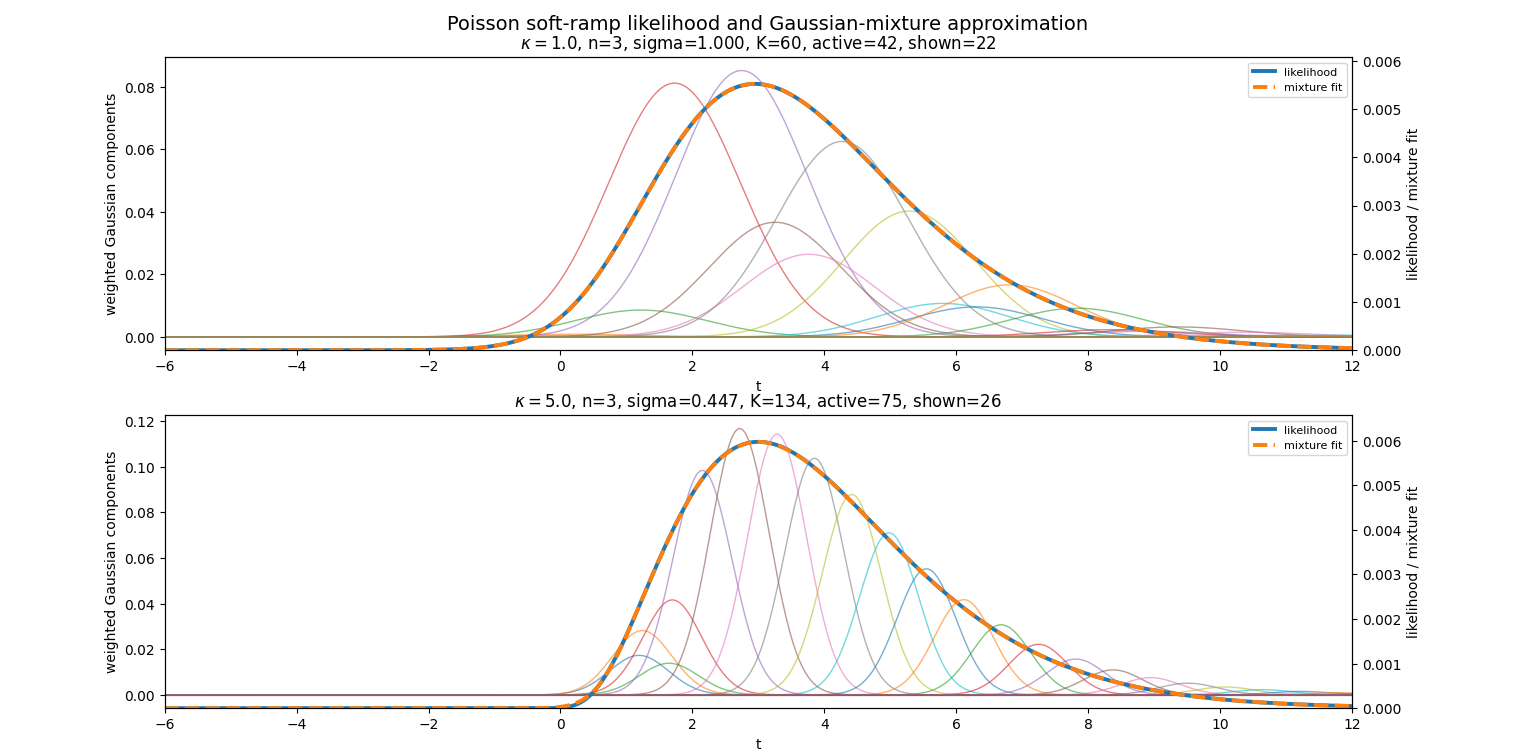
\includegraphics[width=0.99\linewidth]{likelihood_mixture_k1_k5.png}
\end{center}
\vspace{-3mm}
\captiontext{$n=3$: $\kappa=1$ (top) and $\kappa=5$ (bottom).
Blue is the likelihood; dashed orange is the mixture fit.}
}
\end{minipage}
\hfill
\begin{minipage}[t]{0.483\textwidth}
\vspace{0pt}
\card{Inference: conditional Gaussian updates}{%
Introduce a mixture indicator $z_i$ for each cell. Gibbs sampling
alternates a categorical update and a joint Gaussian field update:
{\posterformula
\[
\Pr(z_i=r\mid f_i,n_i)\propto
w_{n_i r}\mathcal N(f_i;m_{n_i r},s_{n_i}^2),
\]
\[
f\mid z,n\sim\mathcal N\!\left(\nu_z,(Q+D^{-1})^{-1}\right),
\quad D=\operatorname{diag}(s_{n_i}^2),
\]
\[
\nu_z=(Q+D^{-1})^{-1}(Qm+D^{-1}m_z).
\]
}
With fixed counts, $\kappa$, and prior parameters, $D$ is unchanged
when $z$ changes. The factorization of a sparse $Q+D^{-1}$ can be reused.
The sampler targets the mixture-approximated posterior.
}

\card{Synthetic field demonstration}{%
\begin{center}
\begin{minipage}{0.48\linewidth}\centering
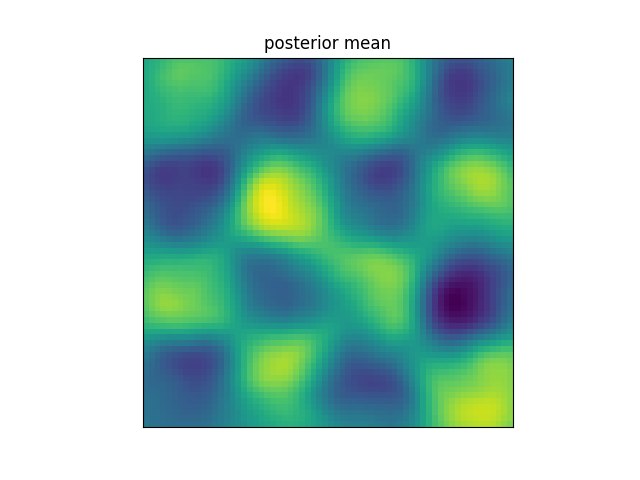
\includegraphics[width=0.98\linewidth,
 trim=140bp 53bp 125bp 50bp,clip]{posterior_mean_k_1.png}\\[3mm]
{\bfseries $\kappa=1$}
\end{minipage}\hfill
\begin{minipage}{0.48\linewidth}\centering
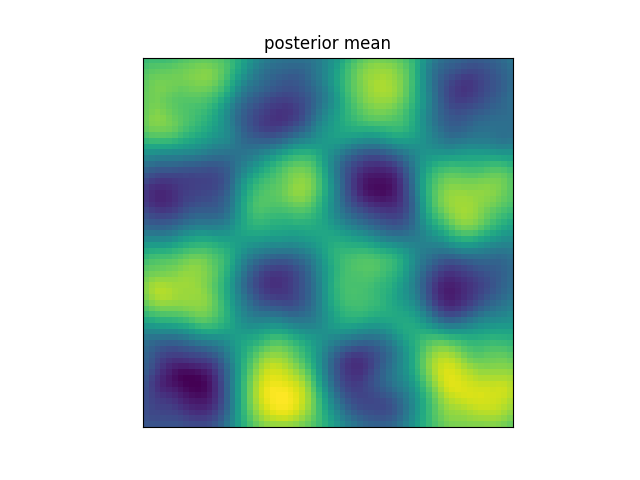
\includegraphics[width=0.98\linewidth,
 trim=140bp 53bp 125bp 50bp,clip]{posterior_mean_k_5.png}\\[3mm]
{\bfseries $\kappa=5$}
\end{minipage}
\end{center}
\captiontext{Posterior mean latent fields after 230 iterations.
The original image color scaling is retained; comparison is qualitative.}
}

\card{Prior-rate sensitivity to $\kappa$}{%
In the synthetic prior experiment, mean cell rates remain close to two,
while larger $\kappa$ produces more cells with low intensity:
\vspace{3mm}
{\fontsize{25}{32}\selectfont
\begin{center}
\begin{tabular}{@{}lrr@{}}
\toprule
$\kappa$ & Mean rate & Fraction below $0.1$\\
\midrule
$0.5$ & $2.046$ & $0.0\%$\\
$1.0$ & $2.033$ & $0.0\%$\\
$2.0$ & $1.979$ & $4.4\%$\\
$5.0$ & $1.938$ & $10.1\%$\\
\bottomrule
\end{tabular}
\end{center}
}%
}

\card{Sampling cost in the supplied experiment}{%
\captiontext{Wall time for 100 yielded samples. These columns use
different links: sigmoid with P\'olya--Gamma (PG) augmentation and
softplus with a fitted mixture.}
\vspace{3mm}
{\fontsize{25}{32}\selectfont
\begin{center}
\begin{tabular}{@{}lrrr@{}}
\toprule
Grid & Sigmoid + PG & Softplus + mixture & PG / mixture\\
\midrule
$16\times16$ & 0.232 s & 0.766 s & 0.30\\
$32\times32$ & 4.889 s & 3.472 s & 1.41\\
$64\times64$ & 119.271 s & 23.663 s & 5.04\\
\bottomrule
\end{tabular}
\end{center}
}
At $64\times64$ the mixture sampler took about one fifth of the PG time
in this experiment; the table is not an accuracy comparison.
}

\card{References}{%
\captiontext{C. Donner and M. Opper (2018).
\emph{Efficient Bayesian Inference of Sigmoidal Gaussian Cox Processes.}
\emph{Journal of Machine Learning Research} \textbf{19}(67), 1--34.
\href{https://jmlr.org/papers/v19/17-759.html}{jmlr.org/papers/v19/17-759.html}.}
\vspace{4mm}
\captiontext{C. Molkenthin, C. Donner, S. Reich, G. Z\"oller,
S. Hainzl, M. Holschneider, and M. Opper (2022).
\emph{GP-ETAS: semiparametric Bayesian inference for the spatio-temporal
epidemic type aftershock sequence model.}
\emph{Statistics and Computing} \textbf{32}, Article 29.
\href{https://doi.org/10.1007/s11222-022-10085-3}
{doi:10.1007/s11222-022-10085-3}.}
}
\end{minipage}

\vfill
\noindent\colorbox{upblue}{%
  \parbox[c][43mm][c]{\textwidth}{%
    \hspace*{13mm}{\color{white}\bfseries\fontsize{30}{37}\selectfont
      Cristina O. Ch\'avez Chong \quad Toni Ludo \quad Matthias Holschneider \hfill
      \href{mailto:cristina.chavez@uni-potsdam.de}
        {\color{white}cristina.chavez@uni-potsdam.de}\hspace*{13mm}}%
  }%
}
\end{document}
